\documentclass[border=2pt]{standalone}
\usepackage[utf8]{inputenc} % Required for inserting images
\usepackage{tikz}
\usepackage{helvet}
\usetikzlibrary{shapes.geometric, arrows}
\pagecolor{white}

%-------------------------defining colorblind friendly colors
% Using pale color scheme in Figure 6
% by Paul Tol https://personal.sron.nl/~pault/
\definecolor{cbblue}{HTML}{BBCCEE}
\definecolor{cbcyan}{HTML}{CCEEFF}
\definecolor{cbgreen}{HTML}{CCDDAA}
\definecolor{cbyellow}{HTML}{EEEEBB}
\definecolor{cbred}{HTML}{FFCCCC}
\definecolor{cbgrey}{HTML}{DDDDDD}

% -------------------------defining nodes
\tikzstyle{input} = [trapezium, trapezium left angle =80, trapezium right angle = 100,
minimum width= 3cm, minimum height=0.5cm, text centered, draw=black, fill=cbblue]
\tikzstyle{process} = [rectangle, minimum width = 3cm, minimum height = 0cm,
text centered, , text width=4cm,draw=black, fill=cbgrey]
\tikzstyle{decision} = [diamond, minimum width = 0cm, minimum height = 0cm,
text centered, , text width=1cm, draw=black, fill=cbcyan]
\tikzstyle{changeclass} = [rectangle, rounded corners, minimum width=3cm, minimum height=1cm,
text centered, draw = black, fill=cbyellow]
\tikzstyle{reject} = [trapezium, trapezium left angle =80, trapezium right angle = 100,
minimum width= 1cm, minimum height=0.5cm, text centered, draw=black, fill=cbred]
\tikzstyle{accept} = [trapezium, trapezium left angle =80, trapezium right angle = 100,
minimum width= 1cm, minimum height=0.5cm, text centered, draw=black, fill=cbgreen]

% -------------------------defining connectors
\tikzstyle{arrow} = [thick,->, >=stealth]
\tikzstyle{line} = [thick,-,>=stealth]
\begin{document}

% ------------------------- tikz image (flow chart)
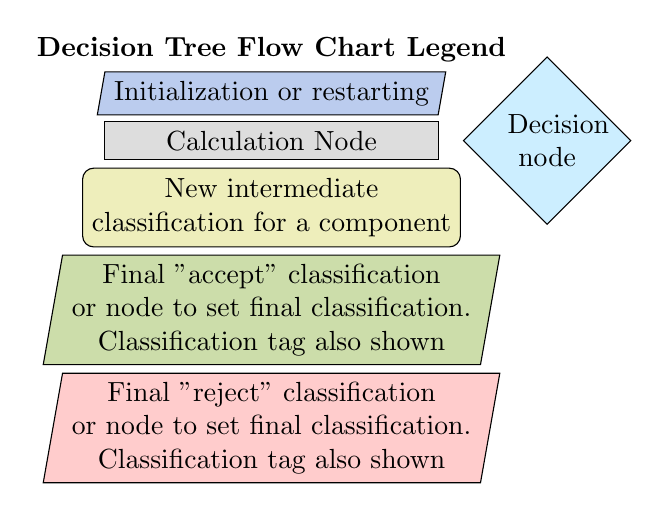
\begin{tikzpicture}[node distance = 1cm]

% ------------------------- nodes -------------------------

% ----- node: 0
\node(0)[input, label={90:\textbf{Decision Tree Flow Chart Legend}}] {Initialization or restarting};
% ----- node: 1
\node(1)[process, below of=0, align=center, yshift=0.4cm] {Calculation Node};
% ----- node: 2
\node(2)[changeclass, below of=1, align=center, yshift=0.15cm] {New intermediate\\classification for a component};
% ----- node: 3
\node(3)[decision, right of=1, xshift=2.5cm, align=center] {Decision node};
% ----- node: 4
\node(4)[accept, below of=2, align=center, yshift=-0.3cm] {Final "accept" classification\\or node to set final classification.\\Classification tag also shown};
% ----- node: 5
\node(5)[reject, below of=4, align=center, yshift=-0.5cm] {Final "reject" classification\\or node to set final classification.\\Classification tag also shown};


\end{tikzpicture}
\end{document}
